\documentclass{beamer}

% --------------------------------------------------------------------
% THEME AND APPEARANCE
% --------------------------------------------------------------------
% Choose a theme for the presentation.
% Popular themes: Madrid, Berlin, Boadilla, CambridgeUS, Copenhagen,
% Darmstadt, Dresden, Frankfurt, Goettingen, Hannover, Ilmenau,
% Juanlespins, Luebeck, Malmoe, Marburg, Montpellier, PaloAlto,
% Pittsburgh, Rochester, Singapore, Szeged, Warsaw.
\usetheme{CambridgeUS}


% Choose a color theme.
% Popular color themes: beaver, beetle, crane, dolphin, dove, fly,
% lily, orchid, rose, seagull, seahorse, whale, wolverine.
\usecolortheme{default}
% add a logo to the title page (optional)
%\titlegraphic{\includegraphics[height=1.5cm]{logo.png}}

% --------------------------------------------------------------------
% PACKAGES
% --------------------------------------------------------------------
\usepackage{tikz}     % For drawing diagrams
\usetikzlibrary{positioning, arrows.meta}
\usepackage{graphicx} % For including images
\usepackage{booktabs} % For professional quality tables
\usepackage{minted}   % For syntax-highlighted code blocks.
                      % This requires the 'pygments' Python package to be installed.
                      % You may need to compile with the -shell-escape flag (e.g., pdflatex -shell-escape main.tex)
\usepackage{hyperref}
\usetikzlibrary{calc}
% --------------------------------------------------------------------
% PRESENTATION METADATA
% --------------------------------------------------------------------
\title[Some Fun With Bevy]{An Overview to Game Development Using Rust}
\subtitle{A Toxic Relationship With Rust}
\author{Marti}
\institute{OmniMeet}
\date{November 25, 2025}

\begin{document}

% --------------------------------------------------------------------
% TITLE PAGE
% --------------------------------------------------------------------
\begin{frame}
  \titlepage
\end{frame}


\AtBeginSection[]
{
  \begin{frame}{Where am I?}
    \tableofcontents[currentsection,currentsubsection]
  \end{frame}
}

\AtBeginSubsection[]
{
  \begin{frame}{Outline}
    \tableofcontents[currentsection,currentsubsection]
  \end{frame}
}
\section{What is Bevy?}
% make me a slide with bevy logo and some text about bevy
\begin{frame}{What is Bevy?}
  \frametitle{Bevy Game Engine}
  \begin{columns}[T] % T aligns columns at the top
    \begin{column}{0.4\textwidth}
      \includegraphics[width=\textwidth]{bevy_logo.png} % Placeholder for Bevy logo
    \end{column}
    \begin{column}{0.6\textwidth}
      \textbf{Bevy} is an open-source data-driven game engine built in Rust.
      \begin{itemize}
        \item It emphasizes simplicity, modularity, and performance.
        \item Bevy uses an Entity-Component-System (ECS) architecture.
        \item It provides a range of features including 2D/3D rendering, audio, input handling, and more.
      \end{itemize}
    \end{column}
  \end{columns}
\end{frame}
\section{Why use Bevy for game development?}
\begin{frame}{Why use Bevy for game development?}
  \frametitle{Advantages of Bevy}
  \begin{itemize}
    \item \textbf{Rust Language}: Memory safety without garbage collection, zero-cost abstractions, and fearless concurrency.
    \item \textbf{ECS Architecture}: Promotes clean code organization, scalability, and high performance through data-oriented design.
    \item \textbf{Cross-Platform}: Deploy to Windows, macOS, Linux, Web (WASM), iOS, and Android from a single codebase.
    \item \textbf{Open Source}: MIT/Apache 2.0 licensed, actively maintained by a vibrant community.
    \item \textbf{Code-Driven}: Pure code workflow with no lock-in to proprietary editors (Official editor \href{https://bevy.org/news/bevys-fifth-birthday/\#bevy-editor-design}{in development}).
    \item \textbf{Modular Design}: Use only what you need - built as a collection of plugins you can mix and match.
  \end{itemize}
\end{frame}
\begin{frame}{Why not use Godot or Unity?}
  \frametitle{Bevy vs Other Engines}

    \begin{center}
    \begin{tabular}{ccc}
      \includegraphics[width=0.25\textwidth]{godot-logo.png} &
      \includegraphics[width=0.25\textwidth]{unity-logo.png} &
      \includegraphics[width=0.25\textwidth]{unreal-engine-logo.png} \\
      \href{https://godotengine.org/}{Godot} &
      \href{https://unity.com/}{Unity} &
      \href{https://www.unrealengine.com/}{Unreal Engine}
    \end{tabular}
  \end{center}
  \begin{itemize}
    \item \textbf{Lightweight}: Lightweight compared to larger engines.
    \item \textbf{Flexibility}: More control over low-level systems and architecture.
    \item \textbf{Paradigm}: ECS is still not really popular in general.
  \end{itemize}
\end{frame}
\section{How does Bevy works?}
\subsection{ECS Architecture}

\begin{frame}{ECS Architecture}
  \frametitle{Entity-Component-System (ECS)}
  
  \begin{center}
    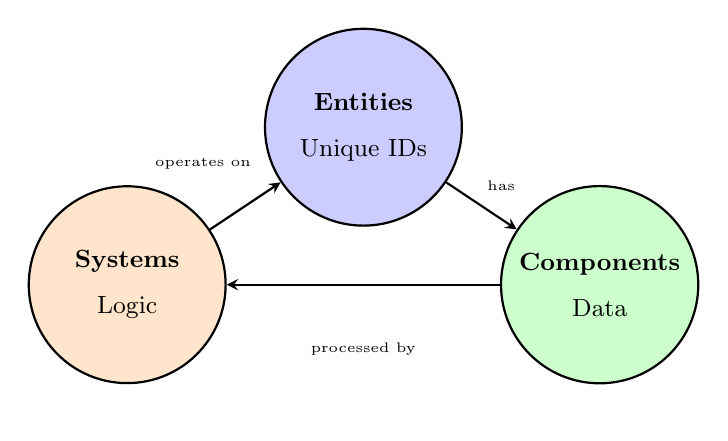
\begin{tikzpicture}[
      node distance=3.5cm,
      every node/.style={draw, circle, minimum size=2.5cm, align=center, font=\small, thick},
      arrow/.style={->, >=stealth, thick}
    ]
      \node[fill=blue!20] (entity) at (0,2) {\textbf{Entities}\\[0.2cm]Unique IDs};
      \node[fill=green!20] (component) at (3,0) {\textbf{Components}\\[0.2cm]Data};
      \node[fill=orange!20] (system) at (-3,0) {\textbf{Systems}\\[0.2cm]Logic};
      
      \draw[arrow] (entity) -- (component) node[midway, above right, draw=none, minimum size=0] {\tiny has};
      \draw[arrow] (component) -- (system) node[midway, below, draw=none, minimum size=0] {\tiny processed by};
      \draw[arrow] (system) -- (entity) node[midway, above left, draw=none, minimum size=0] {\tiny operates on};
    \end{tikzpicture}
  \end{center}
    
  \vspace{-0.6cm}
  \begin{columns}[T]
    \begin{column}{0.3\textwidth}
      \centering
      \colorbox{blue!20}{\parbox{0.9\textwidth}{
        \centering
        \textbf{\large Entities}\\[0.3cm]
        \small Unique identifiers representing objects in the game world
      }}
    \end{column}
    \begin{column}{0.3\textwidth}
      \centering
      \colorbox{green!20}{\parbox{0.9\textwidth}{
        \centering
        \textbf{\large Components}\\[0.3cm]
        \small Data containers that hold attributes of entities
      }}
    \end{column}
    \begin{column}{0.3\textwidth}
      \centering
      \colorbox{orange!20}{\parbox{0.9\textwidth}{
        \centering
        \textbf{\large Systems}\\[0.3cm]
        \small Logic that operates on entities with specific components
      }}
    \end{column}
  \end{columns}
\end{frame}

\subsection{Imagine that you have a cow (Conceptual Example)}
% imagina que tu madre se queda sin dientes i viene juanxu i te dice, una cumbia?
\begin{frame}
  \includegraphics[width=0.4\textwidth]{cow.png} % Placeholder for an image illustrating ECS  
\end{frame}

\begin{frame}
  \frametitle{Traditional OOP Approach}
  \framesubtitle{Shitty Inheritance Hierarchy}
  
  \begin{columns}[c]
    \begin{column}{0.4\textwidth}
      \centering
      \includegraphics[width=0.9\textwidth]{cow.png}
    \end{column}

    \begin{column}{0.8\textwidth}
      \resizebox{0.8\textwidth}{!}{

        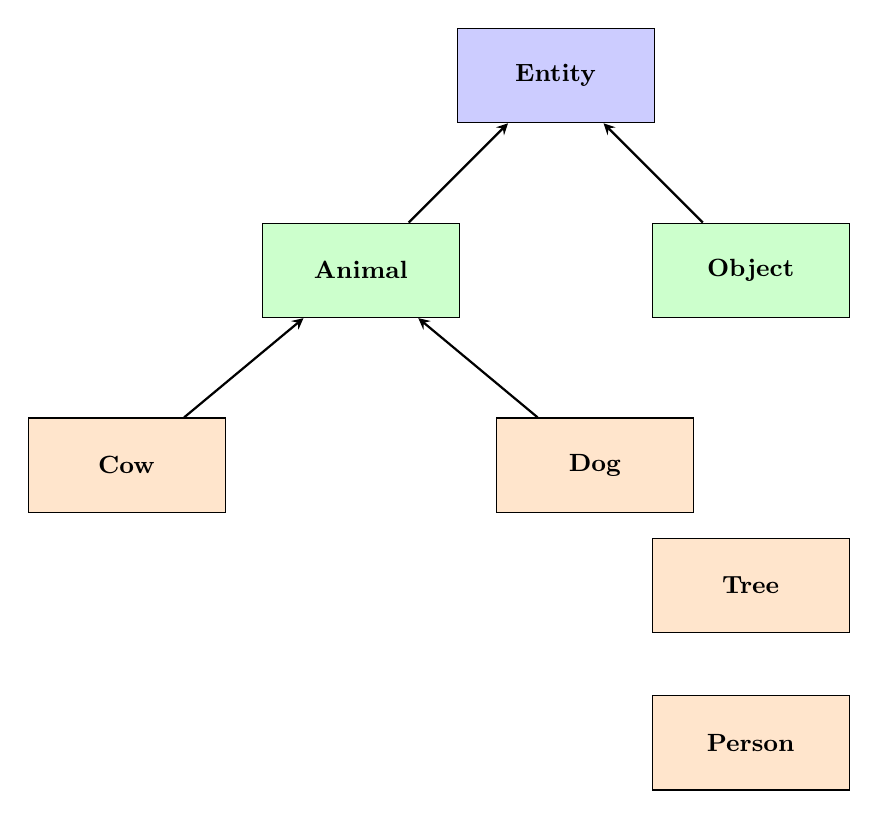
\begin{tikzpicture}[
          node distance=3.5cm and 1cm,
          class/.style={rectangle, draw, fill=blue!10, minimum width=2.5cm, minimum height=1.2cm, align=center, font=\small},
          arrow/.style={->, >=stealth, thick}
        ]
          % Top level
          \node[class, fill=blue!20] (entity) {\textbf{Entity}};
          
          % Second level
          \node[class, fill=green!20, below left of=entity] (animal) {\textbf{Animal}};
          \node[class, fill=green!20, below right of=entity] (object) {\textbf{Object}};
          
          % Third level - under Animal
          \node[class, fill=orange!20, below left of=animal, xshift=-0.5cm] (cow) {\textbf{Cow}};
          \node[class, fill=orange!20, below right of=animal, xshift=0.5cm] (dog) {\textbf{Dog}};
          
          % Third level - under Object
          \node[class, fill=orange!20, below of=object, yshift=-0.5cm] (tree) {\textbf{Tree}};
          \node[class, fill=orange!20, below of=object, yshift=-2.5cm] (person) {\textbf{Person}};
          
          % Arrows
          \draw[arrow] (animal) -- (entity);
          \draw[arrow] (object) -- (entity);
          \draw[arrow] (cow) -- (animal);
          \draw[arrow] (dog) -- (animal);
      \end{tikzpicture}
      }
    \end{column}
  \end{columns}
\end{frame}



\begin{frame}
  \frametitle{ECS Approach}
  \framesubtitle{Nice GIGACHAT and Clean Composition}
  \begin{columns}[c]
    \begin{column}{0.4\textwidth}
      \centering
      \includegraphics[width=0.9\textwidth]{cow.png}
    \end{column}

    \begin{column}{0.8\textwidth}
      
\resizebox{7cm}{!}{
  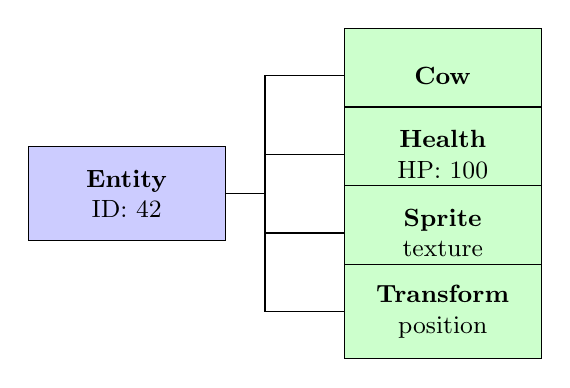
\begin{tikzpicture}[
    node distance=0.4cm and 2cm,
    class/.style={rectangle, draw, fill=blue!10, minimum width=2.5cm, minimum height=1.2cm, align=center, font=\small},
    arrow/.style={-, thick}
  ]
    % Entity at the left
    \node[class, fill=blue!20] (entity) {\textbf{Entity}\\ID: 42};
    
    % Vertical line from entity
    \draw (entity.east) -- ++(0.5,0) coordinate (branch);
    
    % Components on the right
    \node[class, fill=green!20, right=1.5cm of entity, yshift=1.5cm] (cow) {\textbf{Cow}};
    \node[class, fill=green!20, right=1.5cm of entity, yshift=0.5cm] (health) {\textbf{Health}\\HP: 100};
    \node[class, fill=green!20, right=1.5cm of entity, yshift=-0.5cm] (sprite) {\textbf{Sprite}\\texture};
    \node[class, fill=green!20, right=1.5cm of entity, yshift=-1.5cm] (location) {\textbf{Transform}\\position};
    
    % Tree-style connections
    \draw (branch) |- (cow.west);
    \draw (branch) |- (health.west);
    \draw (branch) |- (sprite.west);
    \draw (branch) |- (location.west);
  \end{tikzpicture}
}
    \end{column}
  \end{columns}
\end{frame}


\subsection{How Entitis Work in Bevy?}
\begin{frame}{How Entities Work in Bevy}
  \frametitle{Entities in Bevy}
  
  \begin{center}
    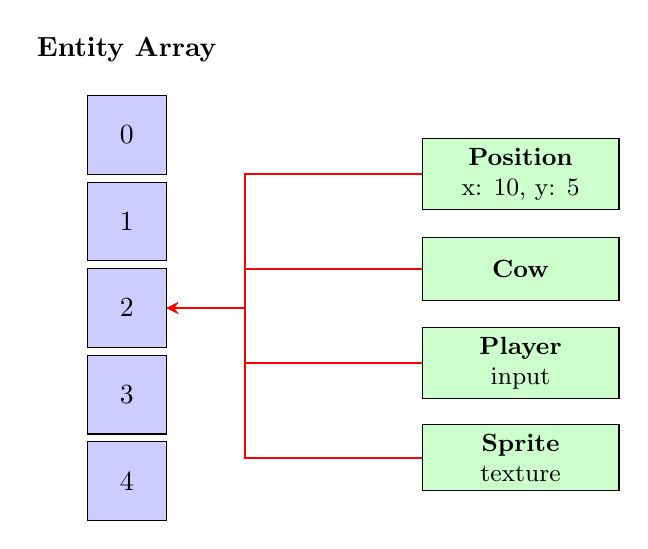
\begin{tikzpicture}[
      entity/.style={rectangle, draw, fill=blue!20, minimum width=1cm, minimum height=1cm},
      component/.style={rectangle, draw, fill=green!20, minimum width=2.5cm, minimum height=0.8cm, align=center, font=\small},
      arrow/.style={->, >=stealth, thick, red}
    ]
      % Vertical Array of entities
      \node[entity] (e0) at (0,0) {0};
      \node[entity] (e1) at (0,-1.1) {1};
      \node[entity] (e2) at (0,-2.2) {2};
      \node[entity] (e3) at (0,-3.3) {3};
      \node[entity] (e4) at (0,-4.4) {4};
      
      % Label for the array
      \node[above=0.3cm of e0] {\textbf{Entity Array}};
      
      % Components stacked vertically on the right
      \node[component] (position) at (5,-0.5) {\textbf{Position}\\x: 10, y: 5};
      \node[component] (cow) at (5,-1.7) {\textbf{Cow}};
      \node[component] (player) at (5,-2.9) {\textbf{Player}\\input};
      \node[component] (sprite) at (5,-4.1) {\textbf{Sprite}\\texture};
      
      % Arrows from components to entity 2
      \coordinate (branch) at (1.5,-2.2);
      \draw[arrow] (position.west) -| (branch) -- (e2.east);
      \draw[arrow] (cow.west) -| (branch) -- (e2.east);
      \draw[arrow] (player.west) -| (branch) -- (e2.east);
      \draw[arrow] (sprite.west) -| (branch) -- (e2.east);
    \end{tikzpicture}
  \end{center}
\end{frame}


\subsection{Bevy's Rendering Pipeline}
\begin{frame}{Bevy's Rendering Pipeline}
  \frametitle{Rendering in Bevy}
  
  \begin{center}
    \scriptsize For more info check \href{https://bevy-cheatbook.github.io/gpu/intro.html}{https://bevy-cheatbook.github.io/gpu/intro.html}
  \end{center}
  
  \begin{center}
    \resizebox{\textwidth}{!}{
    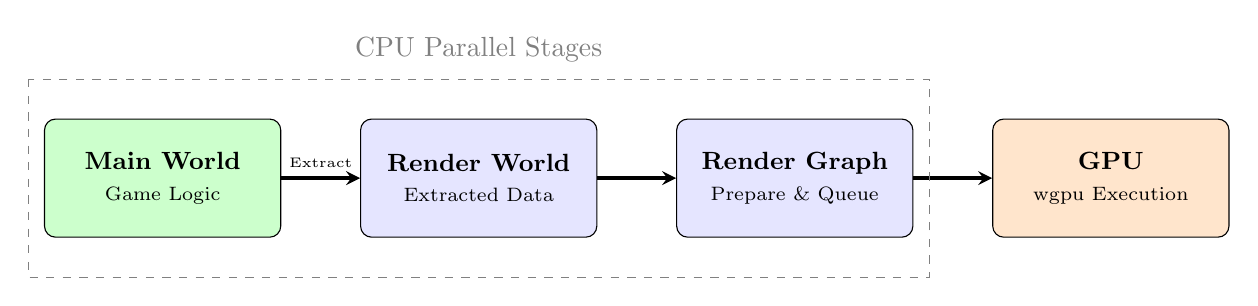
\begin{tikzpicture}[
      node distance=1cm,
      block/.style={rectangle, draw, fill=blue!10, minimum width=3cm, minimum height=1.5cm, align=center, rounded corners, font=\small},
      arrow/.style={->, >=stealth, very thick}
    ]
      % Nodes
      \node[block, fill=green!20] (main) {\textbf{Main World}\\\scriptsize Game Logic};
      \node[block, right=of main] (extract) {\textbf{Render World}\\\scriptsize Extracted Data};
      \node[block, right=of extract] (prepare) {\textbf{Render Graph}\\\scriptsize Prepare \& Queue};
      \node[block, fill=orange!20, right=of prepare] (gpu) {\textbf{GPU}\\\scriptsize wgpu Execution};
      
      % Arrows
      \draw[arrow] (main) -- node[above, font=\tiny] {Extract} (extract);
      \draw[arrow] (extract) -- (prepare);
      \draw[arrow] (prepare) -- (gpu);
      
      % Frame for CPU vs GPU
      \draw[dashed, gray] ($(main.north west)+(-0.2,0.5)$) rectangle ($(prepare.south east)+(0.2,-0.5)$);
      \node[above, gray] at ($(extract.north)+(0,0.6)$) {CPU Parallel Stages};
      
    \end{tikzpicture}
    }
  \end{center}
  
  \vspace{0.3cm}
  \begin{itemize}
    \item \textbf{Pipelined}: Rendering logic runs in parallel with the next frame's game logic.
    \item \textbf{wgpu}: Modern backend supporting Vulkan, Metal, DX12, and WebGPU.
    \item \textbf{Render Graph}: Modular and customizable rendering passes.
  \end{itemize}
\end{frame}

\begin{frame}[plain]
  \begin{tikzpicture}[remember picture,overlay]
    \node[at=(current page.center)] {
      \includegraphics[width=\paperwidth, height=\paperheight]{pipelined-rendering.png}
    };
  \end{tikzpicture}
\end{frame}

\subsection{Resources and Components}
\begin{frame}{Resources and Components in Bevy}
  \frametitle{Resources vs Components}
  
  \begin{columns}[T]
    \begin{column}{0.48\textwidth}
      \centering
      \colorbox{green!20}{\parbox{0.9\textwidth}{
        \centering
        \textbf{\large Components}\\[0.2cm]
        \small Data attached to entities
      }}
      \vspace{0.3cm}
      \begin{itemize}
        \item Attached to specific entities
        \item Multiple instances exist
        \item Defines object properties
        \item Examples: Position, Health, Sprite
      \end{itemize}
    \end{column}
    
    \begin{column}{0.48\textwidth}
      \centering
      \colorbox{orange!20}{\parbox{0.9\textwidth}{
        \centering
        \textbf{\large Resources}\\[0.2cm]
        \small Global unique data
      }}
      \vspace{0.3cm}
      \begin{itemize}
        \item Accessible by all systems
        \item Only one instance exists
        \item Defines world state
        \item Examples: Time, Score, AssetServer
      \end{itemize}
    \end{column}
  \end{columns}
\end{frame}


\subsection{How to access Resources and Components in Systems?}

\begin{frame}[fragile]{Organizing Code}
  \frametitle{Creating a Plugin}     
  \begin{minted}[fontsize=\small]{rust}
use bevy::prelude::*;

#[derive(Resource, Default)]
struct Score(u32);

pub struct GamePlugin;

impl Plugin for GamePlugin {
    fn build(&self, app: &mut App) {
        app.init_resource::<Score>()
           .add_systems(Startup, setup)
           .add_systems(Update, update_score);
    }
}

fn setup() { println!("Game Started"); }
fn update_score(mut score: ResMut<Score>) { score.0 += 1; }
  \end{minted}
\end{frame}

\begin{frame}[fragile]{Accessing Resources and Components in Systems}
  \frametitle{Bevy System Parameters}     
  \begin{minted}[fontsize=\small]{rust}
use bevy::prelude::*;
fn my_system(
    mut query: Query<&mut Transform>, // Access Components
    time: Res<Time>,                  // Access Resource
) {
    for mut transform in query.iter_mut() {
        transform.translation.x += time.delta_seconds() * 100.0;
    }
}
  \end{minted}
\end{frame}

% spawn entities
\subsection{Spawning Entities with Components}
\begin{frame}[fragile]{Spawning Entities with Components}
  \frametitle{Creating Entities in Bevy}     
  \begin{minted}[fontsize=\small]{rust}
use bevy::prelude::*;
fn spawn_entity(mut commands: Commands) {
    commands.spawn((
        Transform::default(),
        Sprite::default(),
        Health(100),
    ));
}
  \end{minted}
\end{frame}

\begin{frame}[fragile]{Spawning Entities with Components}
  \frametitle{Querying Entities in Bevy with some logic}     
  \begin{minted}[fontsize=\small]{rust}
fn query_enemies(query: Query<Entity, (With<Health>, Without<Cow>)>) {
    for enemy in query.iter() {
        println!("Found enemy entity: {:?}", enemy);
    }
}
  \end{minted}
\end{frame}

\section{Building a simple game with Bevy.}
\begin{frame}
  \frametitle{Building a Simple Game with Bevy}
  \begin{center}
    \Huge The Adventures of Ketamine the Cow
  \end{center}
\end{frame}

\section{Building a simple game with Bevy.}
% only a name, no code needed
\begin{frame}
  \frametitle{Building a Simple Game with Bevy}
  \begin{center}
    \Huge The Adventures of Ketamine the Cow
  \end{center}
\end{frame}  

\section{Conclusion}

\begin{frame}{Conclusion}
  \frametitle{Thank You!}
  
  \begin{center}
    \Huge Q\&A
  \end{center}
  
  \vspace{0.5cm}
  \begin{columns}
    \begin{column}{0.5\textwidth}
      \centering
      \includegraphics[width=0.8\textwidth]{receta-queso-gouda.jpg}
    \end{column}
    \begin{column}{0.5\textwidth}
      \centering
      \includegraphics[width=0.8\textwidth]{fuet.jpeg}
    \end{column}
  \end{columns}

  \vspace{0.3cm}
  \begin{center}
    \Large Queso y Ambutido
  \end{center}
\end{frame}


\end{document}


